%% Lee
%% In dissertation, change 
%    section* to chapter 
%    subsection* to section
%    subsubsection* to subsection

% #######################################################################################################################################
% >>>>>>>>>>>>>>>>>>>>>>>>>>> Results <<<<<<<<<<<<<<<<<<<<<<
\chapter{Results}
\label{sec:Results}
The objective of this work was to design a system able to accelerate multiple disparate \acp{ann} in embedded systems.
\iffalse
This means systems that are not designed to process multiple requests of essentially the same operation.
\fi
Given that these systems cannot effectively utilize \ac{sram}, the main objective was to demonstrate a system that can operate efficiently using a customized \ac{3ddram} with a wide data-bus.
\iffalse
The implemented system decodes instructions, sends configuration to various functions, pre-fetches and pipelines data.
This parallelism allows the system to constantly stream data while results from previous operations are being processed.
\fi

\ac{3dic} technology was exploited, including \ac{3ddram}, because a major theme of this work is that \ac{3dic} provides many benefits, including reduced energy use, lower area requirements, and high bandwidth. 
The bandwidth boost can be significantly increased by using a customized \ac{dram}.
\iffalse
To demonstrate such a system, this work targeted \ac{3dic} technology including \ac{3ddram}. This work proposes that if a system can be purely in \ac{3dic}, the system can take advantage of the benefits
of \ac{3dic} which includes reduced energy, area and high bandwidth.
In addition, this work proposes that given the system is \ac{3dic}, then a customized \ac{dram} would provide a significant bandwidth boost over typical implementations using standard DRAM.
\fi
\iffalse
To maintain a purely \ac{3dic} architecture, the area of the system Manager and Processing Engine had to stay within the physical footprint of the \ac{3ddram}.
\fi
Therefore, it was necessary to show that the proposed system can maintain the required data bandwidth while staying within the physical footprint of the \ac{3ddram}. 


The target technology node chosen was \SI{28}{\nano\meter}, mainly because it's the technology node employed for some recent \acp{gpu} and other \acp{asic} such as \cite{jouppi2017datacenter}.
The design was synthesized using \SI{65}{\nano\meter} libraries and then scaled to \SI{28}{\nano\meter}.  This was necessary because certain library components were unavailable
in \SI{28}{\nano\meter}.
%There are techonlogy scaling number available \cite{schabel2017energy}, but the scaling numbers used by this work were generated by synthesizing a representative design from this work which did not employ register files.
%The module chosen was the \ac{dram} memory controller.

\section{Power and Area Scaling estimates}
\label{sec:Power and Area Scaling estimates}

Some representative portions of the design were synthesized using \SI{28}{\nano\meter} libraries to obtain scaling numbers.
The area and power results from these synthesis runs are shown in Table \ref{tab:Scaling runs}.  The final scaling numbers are shown in Table \ref{tab:Scaling numbers}.

\begin{table}[h]
  % the [] contains position info e.g. [!t] means here
  \centering
  \captionsetup{justification=centering}

  %\begin{minipage}{1\textwidth}
    \centering
    \begin{subtable}{0.65\textwidth}
        \begin{adjustbox}{width=1\textwidth}
            \footnotesize
            \begin{tabular}{ |c|c|c|c|c|c|  }
              \hline
              %\rowcolor{gray!50}
              %\multicolumn{5}{|c|}{Power } \\
              %\hline
              %\rowcolor{gray!25}
          Node  &   Type & Frequency                              & Internal                & Net switching           & Leakage                  \\
              \hline
          \SI{65}{\nano\meter}  &  Logic &\SI[per-mode=symbol]{100}{\mega\hertz}  & \SI{66.9}{\milli\watt} & \SI{1.53}{\milli\watt} & \SI{2.02}{\nano\watt}  \\  % xls
          \SI{28}{\nano\meter}  &  Logic &\SI[per-mode=symbol]{100}{\mega\hertz}  & \SI{13.2}{\milli\watt} & \SI{1.26}{\milli\watt} & \SI{4.9 }{\micro\watt} \\  % xls
          %\SI{65}{\nano\meter}  &  Logic &\SI[per-mode=symbol]{100}{\mega\hertz}  & \SI{142}{\milli\watt} & \SI{123}{\milli\watt} & \SI{192}{\micro\watt}  \\  % main_mem_cntl
          %\SI{28}{\nano\meter}  &  Logic &\SI[per-mode=symbol]{100}{\mega\hertz}  & \SI{ 28}{\milli\watt} & \SI{100}{\milli\watt} & \SI{22.4}{\milli\watt} \\  % main_mem_cntl
%      Scaling  &                                                 & \num{5.06}              & \num{1.22}              & \num{4.11e-3}            \\
              \hline
            \end{tabular}
        \end{adjustbox}
      \caption{Example logic only design synthesis power}
      \label{tab:Scaling}
    \end{subtable}
    \begin{subtable}{0.65\textwidth}
        \vspace{5mm}
        \begin{adjustbox}{width=1\textwidth}
            \footnotesize
            \begin{tabular}{ |c|c|c|c|c|c|  }
              \hline
              %\rowcolor{gray!50}
              %\multicolumn{5}{|c|}{Power } \\
              %\hline
              %\rowcolor{gray!25}
          Node  & Type      & Frequency                              & Internal                & Net switching           & Leakage                 \\
              \hline
          \SI{65}{\nano\meter}  & Memory    & \SI[per-mode=symbol]{100}{\mega\hertz}  & \SI{2.36}{\milli\watt}  & \SI{0.6}{\micro\watt}  & \SI{5.4}{\pico\watt}    \\   % wu_memory
%          \SI{65}{\nano\meter} & Register  & \SI[per-mode=symbol]{100}{\mega\hertz}  & \SI{61  }{\micro\watt}  & \SI{6  }{\micro\watt}  & \SI{12.6}{\nano\watt}   \\
%          \SI{65}{\nano\meter} & Comb      & \SI[per-mode=symbol]{100}{\mega\hertz}  & \SI{  }{\micro\watt}    & \SI{6  }{\micro\watt}  & \SI{12.6}{\nano\watt}   \\
          \SI{28}{\nano\meter}  & Memory    & \SI[per-mode=symbol]{100}{\mega\hertz}  & \SI{43.8}{\micro\watt}  & NR                     & \SI{443}{\micro\watt}   \\   % wu_memory
%          \SI{28}{\nano\meter} & Logic     & \SI[per-mode=symbol]{100}{\mega\hertz}  & \SI{2.8 }{\micro\watt}  & \SI{0.38}{\micro\watt} & \SI{0.53}{\micro\watt}  \\
%       Scaling &                                                     & \num{5.06}              & \num{1.22}             & \num{4.11e-3}           \\
              \hline
            \end{tabular}
        \end{adjustbox}
      \caption{Example design with memory synthesis power}
      \label{tab:Example design with memory synthesis power}
    \end{subtable}
    \begin{subtable}{0.65\textwidth}
        \vspace{5mm}
        \begin{adjustbox}{width=1\textwidth}
            \footnotesize
            \begin{tabular}{ |c|c|c|c|  }
              \hline
              %\rowcolor{gray!50}
              %\multicolumn{5}{|c|}{Power } \\
              %\hline
              %\rowcolor{gray!25}    % wu_memory                                        1024x50                               
          Node  & Type      & Area from synthesis                                 & Area from Datasheet                                \\
              \hline
          \SI{65}{\nano\meter}  & Logic     & \SI[per-mode=symbol]{879593}{\square\micro\meter}  & NA\\ %\SI[per-mode=symbol]{57014}{\square\micro\meter}    \\
          \SI{28}{\nano\meter}  & Logic     & \SI[per-mode=symbol]{327822}{\square\micro\meter}  & NA\\ %\SI[per-mode=symbol]{20281}{\square\micro\meter}    \\
          \SI{65}{\nano\meter}  & Memory    & \SI[per-mode=symbol]{210230}{\square\micro\meter}  & \SI[per-mode=symbol]{57014}{\square\micro\meter}    \\
          \SI{28}{\nano\meter}  & Memory    & \SI[per-mode=symbol]{75605 }{\square\micro\meter}  & \SI[per-mode=symbol]{20281}{\square\micro\meter}    \\
%      Scaling  &           & \num{5.06}                                         & \num{1.22}                                          \\
              \hline
            \end{tabular}
        \end{adjustbox}
      \caption{Example design area}
      \label{tab:Example design area}
    \end{subtable}
  %\end{minipage}
  \captionsetup{justification=centering, skip=9pt}
  \vspace{0.0cm}
  \caption{Example design area and power}
  \label{tab:Scaling runs}
\end{table}

\begin{table}[h]
  % the [] contains position info e.g. [!t] means here
  \centering
  \captionsetup{justification=centering}
  \begin{minipage}{1\textwidth}
    \centering
    \begin{minipage}{0.85\textwidth}
        \vspace{5mm}
        \begin{adjustbox}{width=1\textwidth}
            \footnotesize
            \begin{tabular}{|>{\centering}m{1cm}|>{\centering}m{1cm}|>{\centering}m{1cm}|>{\centering}m{1.3cm}|>{\centering}m{1.3cm}|>{\centering}m{1cm}|>{\centering}m{1.3cm}|m{1.3cm}|}\cline{3-8}
              %\hline
              %\rowcolor{gray!50}
              %\multicolumn{5}{|c|}{Power } \\
              %\hline
              %\rowcolor{gray!25}  
         \multicolumn{2}{c|}{}                                          & \multicolumn{3}{c|}{Logic power}                                                                  &  \multicolumn{3}{c|}{Memory power}                                                                                                                                  \\\cline{1-8}
         Logic Area                  & Memory Area                      & Internal                            & Net switching                  & Leakage                    & Internal                                                                                                              & Net switching                  & Leakage    \\\cline{1-8}
          \num{2.68}                 & \num{2.78}                       &  \num{5.07}                         & \num{1.21}                     & \num{4.12e-4}              & \num{5.07}\footnote{this number is conservative based on Table \ref{tab:Example design with memory synthesis power}}  & NA                             & NA         \\
              \hline
            \end{tabular}
        \end{adjustbox}
      %\subcaption{Example design area}
      %\label{tab:Example design area}
    \end{minipage}
  \end{minipage}
  \captionsetup{justification=centering, skip=9pt}
  \vspace{0.0cm}
  \captionof{table}{\SI{68}{\nano\meter} to \SI{28}{\nano\meter} scaling numbers}
  \label{tab:Scaling numbers}
\end{table}

\section{Physical Placement}
\label{sec:Physical Placement}

Based on the \ac{diram4} layout shown in Figure \ref{fig:diram4Layout}, the dimensions of the area available for each \ac{ssc} are \SI{1470}{\micro\meter} by \SI{1656}{\micro\meter} or approximately \SI{2.43}{\square\milli\meter}.
Using the logic and memory scaling numbers from Table \ref{tab:Scaling numbers}, the effective dimensions at \SI{65}{\nano\meter} is \SI{2431}{\micro\meter} by \SI{2738}{\micro\meter} providing a design area at \SI{65}{\nano\meter} of approximately \SI{6.66}{\square\milli\meter}.
The area contribution of each block within the Manager and \ac{pe} can be seen in Table \ref{tab:Area contribution}.
\begin{table}[h]
%  \captionsetup{justification=centering, skip=-5pt}
  \captionsetup{justification=centering, skip=3pt}
  \caption{Area contribution}
  \vspace{3pt}
  \label{tab:Area contribution}
  \centering
    % [lr] ~ left align col 0 and right align col 1
    % e.g. 4 columns could be lccr
  \begin{subtable}{1\textwidth}
    \centering
    \begin{adjustbox}{width=0.50\textwidth}
      \begin{tabular}{|c|c|c|}
        \hline
                            % \multicolumn{4}{c}{3D-DRAM Simulation-based estimates}   \\
       \multirow{2}{*}{Block name}    &  \multirow{2}{*}{Instances}        &  \multirow{2}{*}{Percentage contribution}     \\  %\cline{1-1}
                                      &                                    &                                               \\
        \hline  % instead of \midrule %midrule doesnt overlap with column lines
  Memory Controller      & 1&\SI[per-mode=symbol]{20.6}{\percent}  \\ 
        NoC              & 1&\SI[per-mode=symbol]{ 6.9}{\percent}  \\
        Read Control     & 2&\SI[per-mode=symbol]{47.1}{\percent}  \\
        Write Control    & 1&\SI[per-mode=symbol]{ 6.7}{\percent}  \\
      Instruction Proc   & 1&\SI[per-mode=symbol]{ 1.7}{\percent}  \\
      Return Data Proc   & 1&\SI[per-mode=symbol]{ 1.6}{\percent}  \\
      System Controller  & 1&\SI[per-mode=symbol]{ 1.6}{\percent}  \\
        TSV              &NA&\SI[per-mode=symbol]{ 6.9}{\percent}  \\
        Misc             &NA&\SI[per-mode=symbol]{ 6.8}{\percent}  \\
        \hline
      \end{tabular}
    \end{adjustbox}
    \vspace{3pt}
    \captionsetup{justification=centering, skip=10pt}
    \caption{Manager}
    \label{tab:Manager Area Contribution}
  \end{subtable}
  \bigskip
  \begin{subtable}{1\textwidth}
    \centering
    \begin{adjustbox}{width=0.55\textwidth}
      \begin{tabular}{|c|c|c|}
        \hline
                            % \multicolumn{4}{c}{3D-DRAM Simulation-based estimates}   \\
       \multirow{2}{*}{Block name}    &  \multirow{2}{*}{Instances}        &  \multirow{2}{*}{Percentage contribution}     \\  %\cline{1-1}
                                      &                                    &                                               \\
        \hline  % instead of \midrule %midrule doesnt overlap with column lines
     Operation Decode    & 1&\SI[per-mode=symbol]{ 3.1}{\percent}  \\
   Return Data Control   & 1&\SI[per-mode=symbol]{ 1.5}{\percent}  \\
    SIMD Wrapper         & 1&\SI[per-mode=symbol]{15.1}{\percent}  \\
        SIMD             & 1&\SI[per-mode=symbol]{17.9}{\percent}  \\
  Streaming Operations   &32&\SI[per-mode=symbol]{40.0}{\percent}  \\
  Streaming Op Control   & 1&\SI[per-mode=symbol]{ 1.9}{\percent}  \\
 Local Memory + Control\footnote{A small amount of scratchpad memory was provided between \acp{stop} and \ac{simd} but in practice could be much smaller. It is not used in any of the fanin tests.}  & 1&\SI[per-mode=symbol]{16.4}{\percent}  \\ 
        TSV              &NA&\SI[per-mode=symbol]{ 3.7}{\percent}  \\
        Misc             &NA&\SI[per-mode=symbol]{ 0.4}{\percent}  \\
        \hline
      \end{tabular}
    \end{adjustbox}
    \vspace{3pt}
    \captionsetup{justification=centering, skip=10pt}
    \caption{PE}
    \label{tab:PE Area Contribution}
  \end{subtable}
  \end{table}

The layout utilization for the manager and \ac{pe} were \SI{82.3}{\percent} and \SI{53.6}{\percent} respectively.
Those numbers strongly suggest the manager was more challenging to place and route.
To get a sense of the physical feasibility of the system, both the manager and \ac{pe} were placed and routed without \ac{drc} using Synopsys\textregistered ~IC Compiler\texttrademark.
A route congestion analysis was performed which indicated very few congested areas, which was most likely due to the wide datapath nature of the design.
A preliminary place and route for the Manager and \ac{pe} are shown in Figure \ref{fig:Manager and PE Die layouts}. 
The physical placement and congestion of the manager and \ac{pe} suggests a relatively low risk of encountering problems in completing a full detailed place and route.

\begin{figure}[h]
\centering
\begin{subfigure}{.5\textwidth}
  \centering
  \centerline{
    \mbox{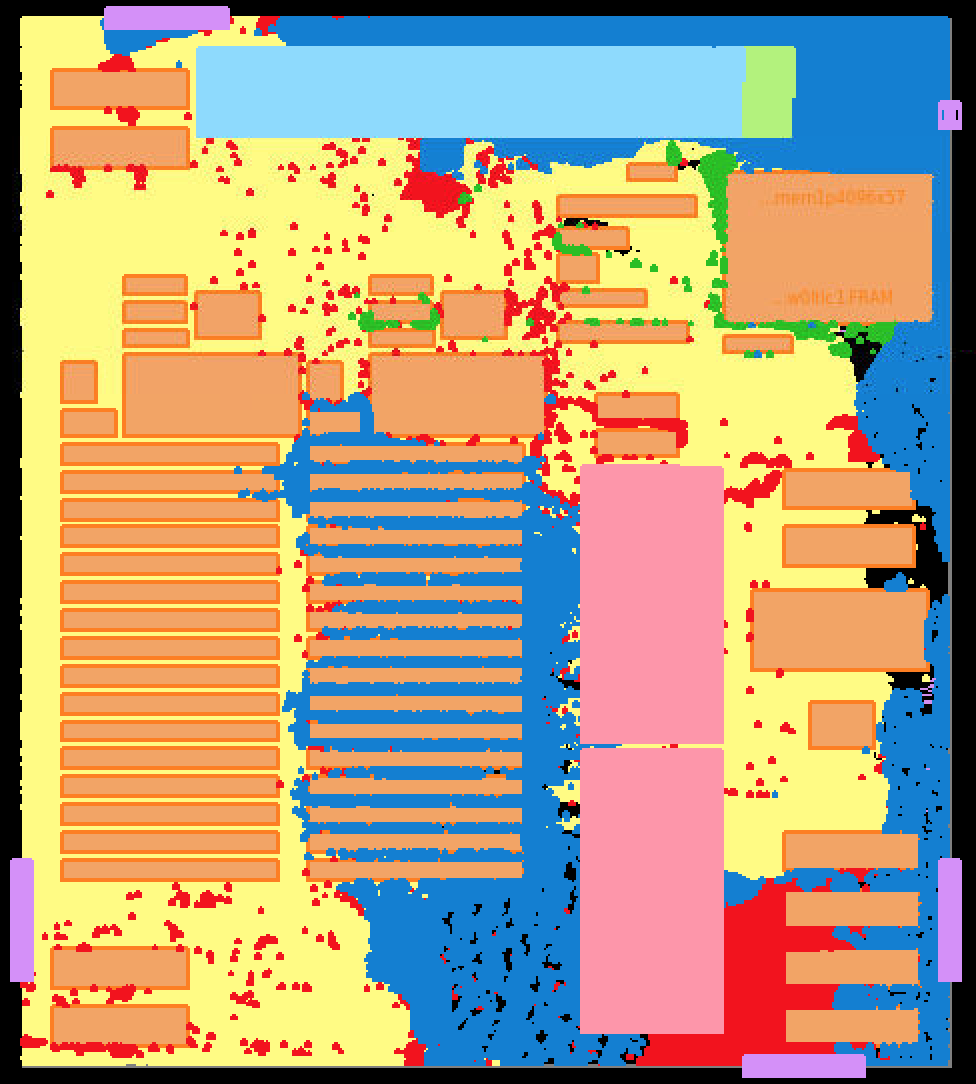
\includegraphics[width=1\linewidth]{ManagerLayout.png}}
  }
  \captionsetup{justification=centering, width=.8\linewidth}
  \caption{Manager}
  %\vspace{40pt}
  \label{fig:managerLayout}
\end{subfigure}%

\bigskip

\begin{subfigure}{.5\textwidth}
  \centering
  \centerline{
    \mbox{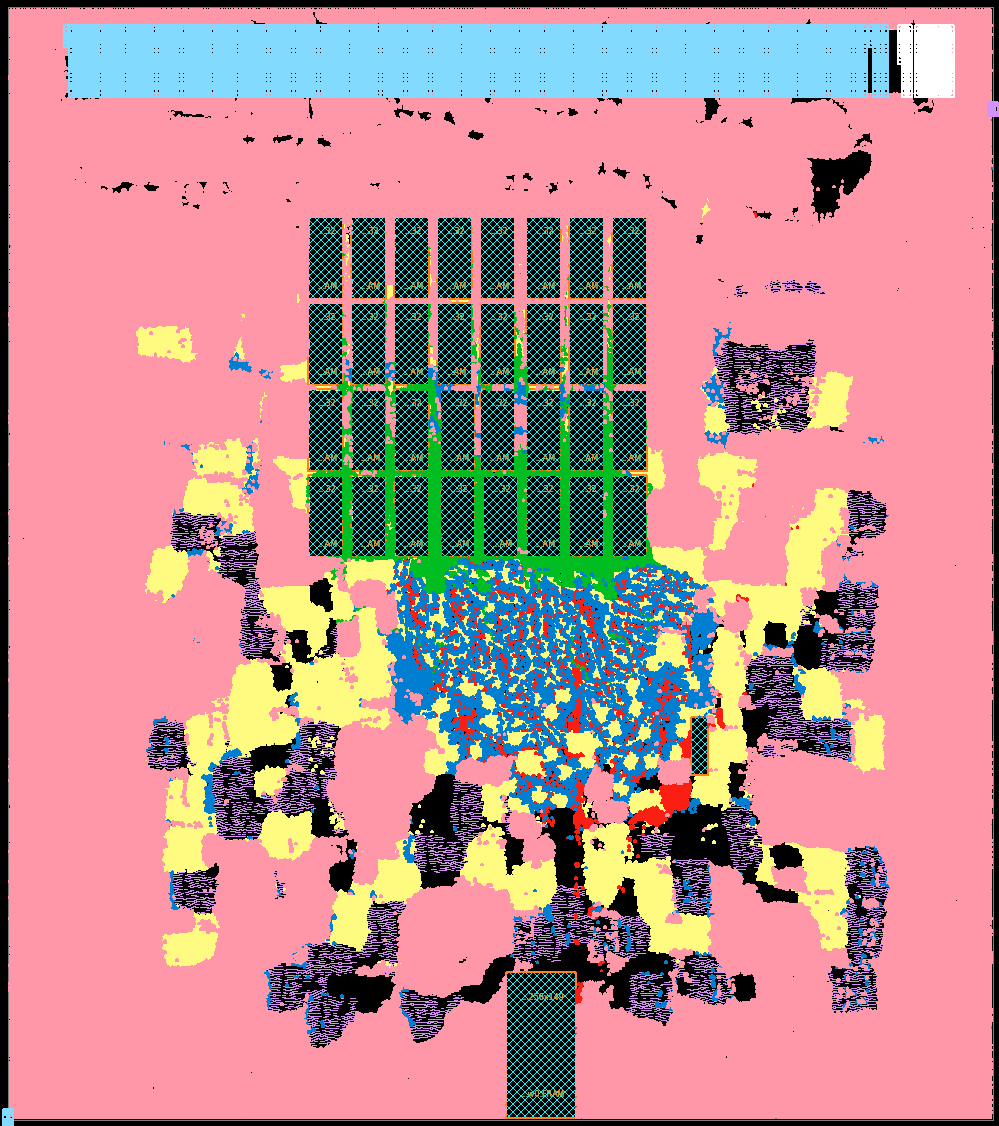
\includegraphics[width=1\linewidth]{PElayout.png}}
  }
  \captionsetup{justification=centering, width=.8\linewidth}
  \caption{PE}
  \label{fig:peLayout}
\end{subfigure}
\captionsetup{justification=centering, width=.9\linewidth}
\caption{Manager and PE Die layouts}
\label{fig:Manager and PE Die layouts}
\end{figure}



\section{Synthesis}
\label{sec:Synthesis}

%The design has been coded . 
An example logic-only design was synthesized using the \SI{28}{\nano\meter} and \SI{65}{\nano\meter} libraries to determine the appropriate frequency scaling between the two technology nodes.
In each case, the frequency was increased until negative timing slack was observed.
This suggested that to achieve an operating frequency of \SI{500}{\mega\hertz} at \SI{28}{\nano\meter}, the design should be synthesized at \SI{65}{\nano\meter} using a frequency of \SI{193}{\mega\hertz}.
All blocks in the system were synthesized using a typical library and no blocks had issues synthesizing using the typical library at this relatively low frequency, suggesting a target frequency of \SI{500}{\mega\hertz} at \SI{28}{\nano\meter} is relatively low risk.


\iffalse
As mentioned previously \eqref{eq:averageBandwidth}, to process multiple useful-sized \acp{ann} requires a sustained bandwidth to the \ac{pe} of the order of tens of \SI[per-mode=symbol]{}{\tera\bit\per\second}.
\fi

%%%%The approximate design targets are shown in Table \ref{tab:DesignTargets}.
%%%%
%%%%\begin{table}[h]
%%%%%  \captionsetup{justification=centering, skip=-5pt}
%%%%  \captionsetup{justification=centering, skip=3pt}
%%%%  \caption{Design targets}
%%%%  \label{tab:DesignTargets}
%%%%  \centering
%%%%%  \begin{center}
%%%%    % [lr] ~ left align col 0 and right align col 1
%%%%    % e.g. 4 columns could be lccr
%%%%    \begin{tabular}{lr}
%%%%      \toprule
%%%%      Parameter         & Target \\
%%%%      \midrule
%%%%      Frequency         & $>$\SI{700}{\MHz}   \\
%%%%      Power             & \SI{\approx 80}{\W}   \\
%%%%      Bandwidth         & \SI[per-mode=symbol]{\approx 64}{\tera\bit\per\second} \\
%%%%      Overall Die Area  & \SI{175}{\mm^2} \\
%%%%      \bottomrule
%%%%    \end{tabular}
%%%%%  \end{center}
%%%%\end{table}


\section{Logic Verification}
\label{sec:Logic Verification}

The primary control and data paths of the system have been simulated in a SystemVerilog environment using Mentor Graphics\textregistered ~ModelSim\texttrademark.
To ensure high bandwidth utilization can be maintained, a group of tests representing convolutional and fully-connected layers was simulated.
The operations simulated were based on the expected lower and upper limits of pre-synaptic fanin. 
These test cases were based on layers similar to CONV2 and FC-7 from \cite{krizhevsky2012imagenet} which represent a pre-synaptic fanin of 225 and 4000 respectively.
Additional test cases were employed representing pre-synaptic fanins of 294, 300, 500 and 1000. Both locally-connected (CONV) and fully-connected (FC) type fanins were tested.
The tests labeled CONV-500 and FC-500 represent convolutional and fully-connected tests respectively, both with a pre-synaptic fanin of 500.
The results showing sustained average bandwidth can be seen in Table \ref{tab:Bandwidth Estimates}.


\begin{table}[h]
  \captionsetup{justification=centering, skip=3pt}
  \caption{Fanin bandwidth tests}
  \vspace{3pt}
  \label{tab:Bandwidth Estimates}
  \centering
    \begin{adjustbox}{width=0.45\textwidth}
      \begin{tabular}{|c|c|c|}
        \cline{1-3}
        \multicolumn{1}{|c|}{\multirow{3}{*}{Test}}                   &                                        \multicolumn{2}{c|}{\multirow{2}{*}{Average Bandwidth at frequency}}                                              \\
                                                                      &                                        \multicolumn{2}{c|}{}                                                                                             \\ \cline{2-3} % still need line even though cells are defined
                                                                      &       \multicolumn{1}{c|}{ \SI{500}{\mega\hertz}}                            & \multicolumn{1}{c|}{ \SI{700}{\mega\hertz}}                               \\ \cline{1-3}
        \multicolumn{1}{|c|}{ CONV2 \cite{krizhevsky2012imagenet}}    & \multicolumn{1}{c|}{ \SI[per-mode=symbol]{\sim 25}{\tera\bit\per\second}}    & \multicolumn{1}{c|}{ \SI[per-mode=symbol]{\sim 35}{\tera\bit\per\second}} \\ %\cline{2-2}
        \multicolumn{1}{|c|}{ CONV-294                           }    & \multicolumn{1}{c|}{ \SI[per-mode=symbol]{\sim 26}{\tera\bit\per\second}}    & \multicolumn{1}{c|}{ \SI[per-mode=symbol]{\sim 37}{\tera\bit\per\second}} \\ %\cline{2-2}
        \multicolumn{1}{|c|}{ CONV-300                           }    & \multicolumn{1}{c|}{ \SI[per-mode=symbol]{\sim 27}{\tera\bit\per\second}}    & \multicolumn{1}{c|}{ \SI[per-mode=symbol]{\sim 37}{\tera\bit\per\second}} \\ %\cline{2-2}
        \multicolumn{1}{|c|}{ CONV-500                           }    & \multicolumn{1}{c|}{ \SI[per-mode=symbol]{\sim 29}{\tera\bit\per\second}}    & \multicolumn{1}{c|}{ \SI[per-mode=symbol]{\sim 41}{\tera\bit\per\second}} \\ %\cline{2-2}
        \multicolumn{1}{|c|}{ CONV-1000                          }    & \multicolumn{1}{c|}{ \SI[per-mode=symbol]{\sim 31}{\tera\bit\per\second}}    & \multicolumn{1}{c|}{ \SI[per-mode=symbol]{\sim 43}{\tera\bit\per\second}} \\ %\cline{2-2}
        \multicolumn{1}{|c|}{ CONV-2500                          }    & \multicolumn{1}{c|}{ \SI[per-mode=symbol]{\sim 32}{\tera\bit\per\second}}    & \multicolumn{1}{c|}{ \SI[per-mode=symbol]{\sim 45}{\tera\bit\per\second}} \\ %\cline{2-2}
        \multicolumn{1}{|c|}{ FC-350                             }    & \multicolumn{1}{c|}{ \SI[per-mode=symbol]{\sim 28}{\tera\bit\per\second}}    & \multicolumn{1}{c|}{ \SI[per-mode=symbol]{\sim 39}{\tera\bit\per\second}} \\ %\cline{2-2}
        \multicolumn{1}{|c|}{ FC-500                             }    & \multicolumn{1}{c|}{ \SI[per-mode=symbol]{\sim 29}{\tera\bit\per\second}}    & \multicolumn{1}{c|}{ \SI[per-mode=symbol]{\sim 41}{\tera\bit\per\second}} \\ %\cline{2-2}
        \multicolumn{1}{|c|}{ FC-1000                            }    & \multicolumn{1}{c|}{ \SI[per-mode=symbol]{\sim 31}{\tera\bit\per\second}}    & \multicolumn{1}{c|}{ \SI[per-mode=symbol]{\sim 43}{\tera\bit\per\second}} \\ %\cline{2-2}
        \multicolumn{1}{|c|}{ FC-7 \cite{krizhevsky2012imagenet} }    & \multicolumn{1}{c|}{ \SI[per-mode=symbol]{\sim 32}{\tera\bit\per\second}}    & \multicolumn{1}{c|}{ \SI[per-mode=symbol]{\sim 45}{\tera\bit\per\second}} \\ \cline{1-3}
        %\hline
      \end{tabular}
    \end{adjustbox}
    \vspace{3pt}
  \end{table}

Considering the baseline system shown in Figure \ref{tab:Baseline Layer Configuration}, the distribution of \ac{an} operations and expected bandwidth are shown in Table \ref{tab:Baseline ANN expected bandwidth}.

\begin{table}[h]
  \captionsetup{justification=centering, skip=3pt}
  \caption{Baseline ANN expected bandwidth}
  \vspace{3pt}
  \label{tab:Baseline ANN expected bandwidth}
  \centering
    \begin{adjustbox}{width=0.85\textwidth}
      \begin{tabular}{|c|c|c|c|c|}
        \hline
    \multirow{2}{*}{Layer}    & \multirow{2}{*}{Operation fanin}  & \multirow{2}{*}{Equivalent test}  & \multirow{2}{*}{Percentage of operations}  &  \multirow{2}{*}{Expected bandwidth}                  \\
                              &                                   &                                   &                                            &                                                       \\\hline
      1                       &   363                             &  CONV-300                         &   44\%                                     &  \SI[per-mode=symbol]{ 11.7 }{\tera\bit\per\second}   \\\cline{1-5}
      2                       &     4                             &  \multicolumn{3}{c|}{Performed during previous layer}                                                                                  \\\cline{1-5}
      3                       &  2400                             &  CONV-2500                        &   28\%                                     &  \SI[per-mode=symbol]{  9.1 }{\tera\bit\per\second}   \\\cline{1-5}
      4                       &     4                             &  \multicolumn{3}{c|}{Performed during previous layer}                                                                                  \\\cline{1-5}
      5                       &  2304                             &  CONV-1000                        &   10\%                                     &  \SI[per-mode=symbol]{  3.0 }{\tera\bit\per\second}   \\\cline{1-5}
      6                       &  3456                             &  CONV-2500                        &   10\%                                     &  \SI[per-mode=symbol]{  3.2 }{\tera\bit\per\second}   \\\cline{1-5}
      7                       &  3456                             &  CONV-2500                        &    7\%                                     &  \SI[per-mode=symbol]{  2.1 }{\tera\bit\per\second}   \\\cline{1-5}
      8                       & 43264                             &  FC-7                             &    1\%                                     &  \SI[per-mode=symbol]{  0.2 }{\tera\bit\per\second}   \\\cline{1-5}
      9                       &  4096                             &  FC-7                             &    1\%                                     &  \SI[per-mode=symbol]{  0.3 }{\tera\bit\per\second}   \\\cline{1-5}
     10                       &  4096                             &  FC-7                             &   <1\%                                     &  \SI[per-mode=symbol]{  0.1 }{\tera\bit\per\second}   \\\cline{1-5}
     \multicolumn{3}{c|}{}                                                                            &  Total                                     &  \SI[per-mode=symbol]{ 29.7 }{\tera\bit\per\second}   \\\cline{4-5}
      \end{tabular}
    \end{adjustbox}
    \vspace{3pt}
  \end{table}

\section{Power Estimates}
\label{sec:Power Estimates}

To estimate power consumption, parasitics were extracted from the preliminary layouts and simulated against CONV2.
The activity file generated by this simulation was used by the Synopsys\textregistered ~Primetime-PX\texttrademark ~power analysis tool to obtain power and bandwidth estimates.
The \ac{dram} accesses were captured and \ac{dram} power dissipation calculated from \cite{tezzaron:diram4}. The power dissipated in the TSVs was estimated from \cite{liu2012compact}.
These estimates were scaled using the scaling numbers from Table \ref{tab:Scaling runs} and used to estimate power dissipation for operating frequencies of \SI{500}{\mega\hertz} and \SI{700}{\mega\hertz} using a \SI{28}{\nano\meter} technology node.
The estimated overall power and per-block contributions are shown in Table \ref{tab:Simulation-based estimates}.

\begin{table}[h]
%  \captionsetup{justification=centering, skip=-5pt}
  \captionsetup{justification=centering, skip=3pt}
  \caption{Power Estimates}
  \vspace{3pt}
  \label{tab:Simulation-based estimates}
  \centering
    % [lr] ~ left align col 0 and right align col 1
    % e.g. 4 columns could be lccr
  \begin{subtable}{1\textwidth}
    \centering
    \begin{adjustbox}{width=0.70\textwidth}
      \begin{tabular}{|c|c|c|c|}
       \hline
       \multirow{2}{*}{Technology node}    &  \multirow{2}{*}{Clock frequency}        &  \multirow{2}{*}{Total expected power}   &  \multirow{2}{*}{Testcase}     \\  %\cline{1-1}
                                           &                                          &                                          &                                \\\hline
       \SI{28}{\nano\meter}                & \SI{500}{\mega\hertz}                    &   \SI{ 75.4}{\watt}                       &  CONV-294\iffalse \SI[per-mode=symbol]{\sim 70}{\percent} \fi \\ %\cline{2-2}
       \SI{28}{\nano\meter}                & \SI{700}{\mega\hertz}                    &   \SI{101.2}{\watt}                       &  CONV-294\iffalse \SI[per-mode=symbol]{\sim 70}{\percent} \fi \\ %\cline{2-2}
        \hline
      \end{tabular}
    \end{adjustbox}
    \vspace{3pt}
    \captionsetup{justification=centering, skip=10pt}
    \caption{Power Dissipation}
    \label{tab:Power dissipation}
  \end{subtable}
  \bigskip
  \begin{subtable}{0.75\textwidth}
    \centering
    \begin{adjustbox}{width=0.55\textwidth}
      \begin{tabular}{|c|c|}
        \hline
       \multirow{2}{*}{Block name}    &  \multirow{2}{*}{Percentage contribution}    \\
                                      &                                              \\\hline
                Manager  & \SI[per-mode=symbol]{56.4}{\percent}  \\ 
                     PE  & \SI[per-mode=symbol]{35.1}{\percent}  \\
                   DRAM  & \SI[per-mode=symbol]{ 6.0}{\percent}  \\
              DRAM TSVs  & \SI[per-mode=symbol]{ 1.5}{\percent}  \\
         Stack Bus TSVs  & \SI[per-mode=symbol]{ 1.0}{\percent}  \\
        \hline
      \end{tabular}
    \end{adjustbox}
    \vspace{3pt}
    \captionsetup{justification=centering, skip=10pt}
    \caption{Power contribution}
    \label{tab:Power Dissipation}
  \end{subtable}
  \end{table}


\section{Summary}
\label{sec:Results summary}

The bandwidth performance shown in Table \ref{tab:Bandwidth Estimates} shows a sustained average bandwidth that meets the requirement shown in Table \ref{tab:Bandwidth and Storage Design Requirements}.
In a full system with data transfers between a host and the \ac{ssc}, there will be idle times but this should have a relatively low impact as it involves mostly input download and result upload.
The focus of the verification environment was the \ac{an} processing which involves the most complex operations in the system, including memory management, flow control, etc.
%The \ac{bootp} process was simulated along with host memory upload and download, mainly to ensure the major data path infrastructure was in place to ensure further features would have minimal impact on the area study.
The list of features implemented and verified is shown in Table \ref{tab:Features implemented}.

\begin{table}[h]
  % the [] contains position info e.g. [!t] means here
  \centering
  \captionsetup{justification=centering}

  \begin{minipage}{1\textwidth}
    \centering
      %\begin{adjustbox}{width=0.85\textwidth}
          \footnotesize
          %\begin{tabular}{|>{\centering}m{1cm}|>{\centering}m{1cm}|>{\centering}m{1cm}|>{\centering}m{1.3cm}|>{\centering}m{1.3cm}|}\cline{1-4}
          %\begin{tabular}{ |>{\centering}m{1.5cm}|>{\centering}m{1.5cm}|>{\centering}m{1.5cm}|m{3cm}|}
          \begin{tabular}{ |m{4cm}|c|c|c|m{3cm}|}
            %\hline
            %\rowcolor{gray!50}
            %\multicolumn{5}{|c|}{Power } \\
            \hline
            %\cline{1-4}
            \rowcolor{gray!25}
 \multicolumn{1}{|c|}{Feature}          &   \multicolumn{2}{c|}{Limitations}                 & Method                  &   \multicolumn{1}{c|}{Comment}                                         \\
            \hline                                                                                                     
        Major processing datapaths      &   \multicolumn{2}{c|}{N}                           & Self checking           &  \multicolumn{1}{c|}{Instructions generated using python scripts}      \\\cline{1-5}
        SIMD Wrapper special functions  &   \multicolumn{2}{c|}{N}                           & \multirow{7}{*}{Visual} &  \multicolumn{1}{c|}{\multirow{7}{*}{Instructions manually generated}} \\\cline{1-3}
        Sync Send                       &   \multicolumn{2}{c|}{Host only}                   &                         &                                                                        \\\cline{1-3}
        Sync Wait                       &   \multicolumn{2}{c|}{Host only}                   &                         &                                                                        \\\cline{1-3}
        Memory Upload                   &   \multicolumn{2}{c|}{Host from \ac{dram}}         &                         &                                                                        \\\cline{1-3}
 \multirow{2}{*}{Memory Download}       &   Solicited   & \multirow{2}{*}{Host to \ac{dram}} &                         &                                                                        \\\cline{2-2}
                                        &   Unsolicited &                                    &                         &                                                                        \\\cline{1-3}
        BootP                           &   \multicolumn{2}{c|}{N}                           &                         &                                                                        \\\cline{1-5}
        %MAC                             &   N                     & Self checking  &  Instructions generated using python scripts \\
            %\hline
          \end{tabular}
      %\end{adjustbox}
  \end{minipage}
  \captionsetup{justification=centering, skip=9pt}
  \vspace{0.0cm}
  \captionof{table}{System features implemented}
  \label{tab:Features implemented}
\end{table}

The design was conservatively coded to ensure there were opportunities for logic reduction. For example, in all the modules \acp{fifo} were employed at primary interfaces and the depths of those \acp{fifo} were generous.
%to avoid debugging flow control issues rather than debugging the system as a whole.
In the design of \acp{fsm}, the number of states was assigned conservatively.
The major interfaces between blocks are all registered, but this is considered a requirement when designing a system of this size.
The area scaling numbers employed are within a reasonable range \cite{schabel2017energy}\footnote{work done by Schabel et al, yet to be published}.
Therefore the place and route feasibility study suggests that embarking on productizing a system based on this work would be relatively low risk.

The power numbers were higher than expected %but the power still within a number that is still considered manageable when the design is run at \SI{500}{\mega\hertz}.
with a power per unit area of \SI[per-mode=symbol]{395}{\milli\watt\per\square\milli\meter\per\giga\hertz} but comparable to the \SI[per-mode=symbol]{389}{\milli\watt\per\square\milli\meter\per\giga\hertz} from \cite{chen2016diannao} and higher than the \SI[per-mode=symbol]{304}{\milli\watt\per\square\milli\meter\per\giga\hertz} from \cite{azarkhish2017neurostream} and the \SI[per-mode=symbol]{191}{\milli\watt\per\square\milli\meter\per\giga\hertz} inferred from \cite{jouppi2017datacenter}.
Therefore there may either be opportunities for power reduction -- such as clock gating -- or a fully completed place and route may result in lower power numbers.
%There is unlikely opportunities for clock gating because most of the logic is active during the processing of an \ac{ann}.
%The power numbers seem high but there is likely room for improvement when productizing the system.

\subsection{Recent state-of-the-art comparison}
\label{sec:State-of-the-art Comparison}
When making comparisons it is important to consider whether a solution meets the requirements and not how high it performs against a particular metric.
This work places emphasis on meeting the requirements and not on maximizing a particular metric.

Both Neurostream \cite{azarkhish2017neurostream}, NeuroCube \cite{kim2016neurocube} and Tetris \cite{gao2017tetris} employ \ac{hmc} \ac{3ddram} to provide capacity and a main memory bandwidth of \SI[per-mode=symbol]{1}{\tera\bit\per\second}.
Neurostream \cite{azarkhish2017neurostream} obtained \SI[per-mode=symbol]{22.7}{\giga OP\per\second\per\watt} and claimed a 3.5X performance improvement over a representative \ac{gpu} while using the same \ac{binary32} number format as this work.
%Neurostream \cite{azarkhish2017neurostream} reported an average performance of \SI[per-mode=symbol]{240}{\giga FLOPS}.
To achieve this performance Neurostream must use its \SI[per-mode=symbol]{1}{\mega\bit} \ac{sram} because the \ac{dram} could only support a sustained \SI[per-mode=symbol]{8}{\giga FLOPS}.

Considering that \ac{dram} bandwidth is the bottleneck, for Neurostream \cite{azarkhish2017neurostream} to meet the bandwidth requirements of this work's target application, it would have to instantiate tens of devices.
This would result in a power dissipation in excess of \SI[per-mode=symbol]{1}{\kilo\watt}.
The \acp{flop} performance and capacity would be impressive but it would far exceed the requirements of the system.
Note that this work achieves \SI[per-mode=symbol]{22.4}{\giga OPs\per\second\per\watt}, which is similar to Neurostream \cite{azarkhish2017neurostream}.

Although both NeuroCube \cite{kim2016neurocube} and Tetris \cite{gao2017tetris} do not support the same \ac{binary32} number format, we can still consider the \ac{dram} bandwidth as being the bottleneck. 
To meet the bandwidth requirements of this work's target application, they would have to instantiate 32 devices.
Even though the power numbers of both NeuroCube \cite{kim2016neurocube} and Tetris \cite{gao2017tetris} do not represent a \ac{binary32} system, 
the resulting power dissipation of \SI[per-mode=symbol]{223}{\watt} and an area of \SI[per-mode=symbol]{544}{sq \milli\meter} still represent an improvement from this work of 3X and 6X respectively.

A similar scenario occurs when comparing Tensor processing unit \cite{jouppi2017datacenter} although the number formats are very different and \cite{jouppi2017datacenter} acknowledges the system relies on batch processing to achieve the very high performance.
It uses \ac{dram} with a bandwidth of \SI[per-mode=symbol]{288}{\giga\bit\per\second} which means this work provides greater than 90 times improvement. 
It should be noted in the case of \cite{jouppi2017datacenter} this is an unfair comparison as they do acknowledge the device relies on batch processing and \ac{ann} parameter ``reuse'' and they also state performance degrades when running fully-connected \acp{ann} and therefore this device is not appropriate for this work's target applications.

The DaDianNao \cite{chen2016diannao} device achieves a higher local memory density by employing \ac{edram} instead of \ac{sram}. A single device has \SI[per-mode=symbol]{288}{\giga\bit} of \ac{edram} with a bandwidth of \SI[per-mode=symbol]{2.48}{\tera\bit\per\second}.
To approach the bandwidth of this work would require ten devices dissipating \SI[per-mode=symbol]{167}{\watt} providing this work a 2.2X improvement.
To approach the storage provided by this work would require over two hundred devices. 
In fact \cite{chen2016diannao} states that to implement one of their example \acp{ann}, which requires \SI[per-mode=symbol]{1.39}{\giga\byte} of storage would require a 36-node system. 
They also reference a 64-node system that they claim would outperform a \ac{gpu} by 450X.
So, even assuming a 64-node DaDianNao system, this work would provide a 25X area improvement and a 14X power dissipation improvement.

The NeuroCube \cite{kim2016neurocube}, Tetris \cite{gao2017tetris}, Neurostream \cite{azarkhish2017neurostream} and DaDianNao \cite{chen2016diannao} most closely match this work and they offer significant speed improvements over \ac{gpu}.
This work provides at least a 6X power improvement and a 3X area improvement over this state of the art, in the target application.
%NeuroCube \cite{kim2016neurocube}, Tetris \cite{gao2017tetris} and Neurostream \cite{azarkhish2017neurostream} and a 40X area and power improvement over DaDianNao \cite{chen2016diannao}, in the target application.



